\section{系统设计}
\subsection{MVC架构}
\subsubsection{表示层}
表示层是平台直接面向用户的界面,直接与用户交互。表示层的主要功能是提供类
型的用户操作界面和操作方案,捕捉和收集用户的输入信息通过表示层和给服务器处理
的信息,从而给前台反馈。用户应该在表示层的功能组中进行所有功能模块的操作。前
端表示层将收集接收到的请求和各种数据,然后将它们传输到应用程序层进行相应的处
理。
\subsubsection{业务逻辑层}
业务逻辑层的主要功能是根据实际的业务规则实现相关的业务逻辑功能。在这个层
中,实现了在表示层中相关的目标服务和功能模块。

\subsubsection{数据层}
数据库管理层的主要职责是管理数据库中不同类型的连接和断开连接,并记录和提
示数据库操作中发生的一些异常,以方便开发人员对相关数据库功能进行测试或调试。
系统的所有功能都与各种信息配置、业务处理数据、系统运行关系和其他信息有关;数
据库文件这些数据和信息,并提供一些基本的搜索接口,以保证数据的可靠性和完整性。


\subsection{系统架构图}

\begin{figure}[!htbp]
	\centering
	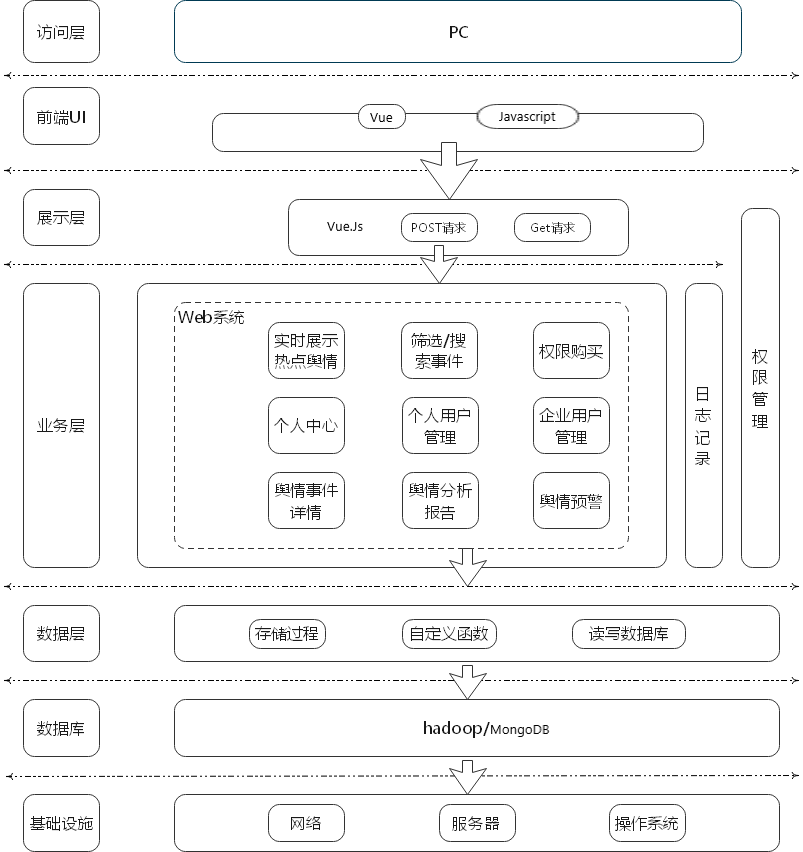
\includegraphics[scale=0.6]{image/a1.png}
\end{figure}